\documentclass[12pt, titlepage]{article}

\usepackage{booktabs}
\usepackage{tabularx}
\usepackage{hyperref}
\usepackage{lscape}
\usepackage{longtable}
\usepackage{graphicx}
\usepackage{float}
\usepackage{comment}
\usepackage[demo]{graphicx}
\usepackage{babel,blindtext}
\hypersetup{
    colorlinks,
    citecolor=black,
    filecolor=black,
    linkcolor=red,
    urlcolor=blue
}
\usepackage[round]{natbib}

%% Comments

\usepackage{color}

\newif\ifcomments\commentstrue %displays comments
%\newif\ifcomments\commentsfalse %so that comments do not display

\ifcomments
\newcommand{\authornote}[3]{\textcolor{#1}{[#3 ---#2]}}
\newcommand{\todo}[1]{\textcolor{red}{[TODO: #1]}}
\else
\newcommand{\authornote}[3]{}
\newcommand{\todo}[1]{}
\fi

\newcommand{\wss}[1]{\authornote{blue}{SS}{#1}} 
\newcommand{\plt}[1]{\authornote{magenta}{TPLT}{#1}} %For explanation of the template
\newcommand{\an}[1]{\authornote{cyan}{Author}{#1}}

%% Common Parts

\newcommand{\progname}{Mechatronics} % PUT YOUR PROGRAM NAME HERE
\newcommand{\authname}{Team \#20, Team Name
\\ Robert Zhu zhul49
\\ Zifan Meng mengz17
\\ Jiahui Chen chenj194
\\ Kelvin Huynh huynhk12
\\ Runze Zhu zhur25
\\ Mirza Nafi Hasan hasanm21} % AUTHOR NAMES                  

\usepackage{hyperref}
    \hypersetup{colorlinks=true, linkcolor=blue, citecolor=blue, filecolor=blue,
                urlcolor=blue, unicode=false}
    \urlstyle{same}
                                


\begin{document}

\title{Verification and Validation Report: \progname} 
\author{\authname}
\date{\today}
	
\maketitle

\pagenumbering{roman}

\section{Revision History}

\begin{tabularx}{\textwidth}{p{3cm}p{2cm}X}
\toprule {\bf Date} & {\bf Version} & {\bf Notes}\\
\midrule
Date 1 & 1.0 & Notes\\
Date 2 & 1.1 & Notes\\
\bottomrule
\end{tabularx}

~\newpage

\section{Symbols, Abbreviations and Acronyms}

\renewcommand{\arraystretch}{1.2}
\begin{tabular}{l l} 
  \toprule		
  \textbf{symbol} & \textbf{description}\\
  \midrule 
  T & Test\\
  \bottomrule
\end{tabular}\\

\wss{symbols, abbreviations or acronyms -- you can reference the SRS tables if needed}

\begin{figure}[H] 
\centering
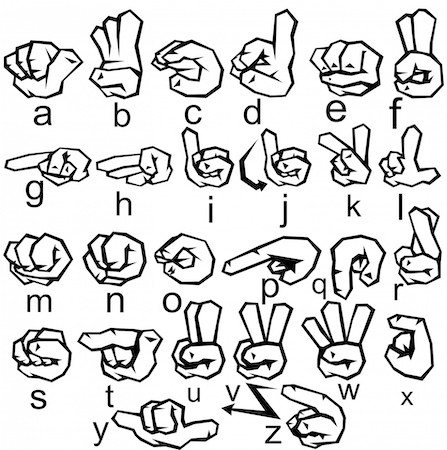
\includegraphics[width=\textwidth,height=0.8\textheight,keepaspectratio]{lower_cases.PNG} 
\caption{Lower Case} 
\label{Fig.Lower Case} 
\end{figure}

\begin{figure}[H] 
\centering
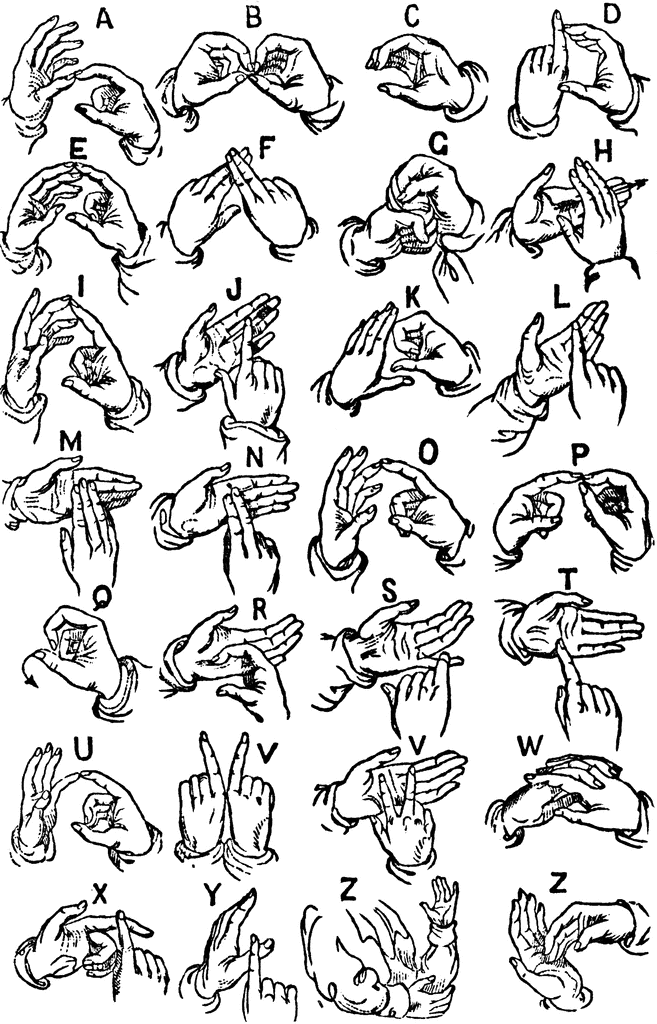
\includegraphics[width=\textwidth,height=0.95\textheight,keepaspectratio]{upper_cases.PNG} 
\caption{Upper Case} 
\label{Fig.Upper Case} 
\end{figure}

\newpage

\tableofcontents

\listoftables %if appropriate

\listoffigures %if appropriate

\newpage

\pagenumbering{arabic}

\section{Purpose}
The purpose of this document is to outline the testing that was done during the development 
of the ASL translator. These tests were conducted to ensure that the ASL translator is able 
to perform as expected and is usable in a real-life setting. This document summarizes the 
results of those tests.

\newpage
\section{Test Cases}
\centerline{Tests for Motion Tracking Module}

\renewcommand{\arraystretch}{1.2}
\noindent \begin{longtable}{p{0.05\linewidth}|p{0.17\linewidth}|p{0.11\linewidth}|p{0.15\linewidth}|p{0.15\linewidth}|p{0.15\linewidth}|p{0.08\linewidth}}
\hline
\textbf{ID} & \textbf{Description} & \textbf{Req Ref} & \textbf{Input} & \textbf{Expected Output} & \textbf{Actual Output} & \textbf{Result}\\
\hline
A1 & Testing for joint tracking when hiding joints & MLFR1, MLFR5, NFR2 & Hand Gesture for “m” and “n” (covering thumb) & Able to recognize hidden joints & Able to recognize hidden joints & Pass\\ \hline
A2 & Testing hand detection for hand at the edges of the camera detection area & CFR1 & Hand gesture for “a”, “b”, “c” & a b c & a b c & Pass\\ \hline
A3 & Testing if joint lines are properly aligned with the user’s joints and move accordingly at the center & MLFR1, MLFR6, NFR2 & Moving hand from one side of the screen to the other in rapid succession & Able to overlay joint lines on user’s hand continually and is centered on the hand & Able to overlay joint lines on user’s hand continually and is centered on the hand & Pass\\ \hline
A4 & Testing if a joint overlay will be placed on more than two hands & MLFR1, MLFR3, NFR2 & Having a third hand in the frame after the initial two & Unable to detect the third hand & Unable to detect the third hand & Pass\\ \hline
A5 & Testing if detected joints are from one individual (the user) & MLFR1, NFR1, NFR3 & Have two people with one hand each in the frame & Detects the hand from one person as opposed to two & Detects both the hands of both people & Fail\\ \hline
A6 & Testing hand detection at a distance of 2 m & CFR1 & Hand gesture for “a”, “b”, “c” & a b c & a b c & Pass\\ \hline
A7 & Testing hand detection with multiple hands & CFR1 & Hand gestures for “z”, “x”, “y” & z x y & z x y & Pass\\ \hline
A8 & Testing for joint tracking when overlapping hands & MLFR1, MLFR3, MLFR5 & Hand Gesture for “S”, “M”, “N”, “R” & Able to separate different hand joints from each other & Able to separate different hand joints from each other & Pass\\ \hline
A9 & Switching from translating mode to training mode stop detecting hand gestures & N/A & Pressing either 2 or 3 & The interface no longer tries to record hand motion & The interface no longer tries to record hand motion & Pass\\ \hline
A10 & Testing for precision tracking & MLFR1 & Making small rotations and tremors & The joint overlay makes small movements & The joint overlay makes small movements & Pass\\ \hline
A11 & Testing for gesture recognition if the hands hand in placing with different angles & CFR1 & Hand gestures for “a”, “b”, “c” with different angles for the position of the hand & “a”, “b”, “c” & “a”, “b”, “c” & Pass\\ \hline
A12 & Testing for occlusion handling & MLFR1 & Partially hiding half of the hand behind a desk & The joint overlay is able to predict the rest of the hand & Joints overlay becomes disjointed and stretches & Fail\\ \hline
A13 & Testing the durability for accuracy and reliability & NFR1, MLFR1 & Keeping the program open for over an hour and testing for similar results & The joint overlay works as intended & The frame rate decreased leading to poor performance & Fail\\ \hline
A14 & User testing for different hand sizes and shapes & MLF1 & Using different people’s hands to test the accuracy of the string “a”, “”b”, “c”, “d” & Able to translate a b c d everytime & Able to translate a b c d everytime & Pass
\hline
\caption{Tests for Motion Tracking Module}
\end{longtable}

\newpage
\centerline{Tests for Coordinate Normalization Module}

\renewcommand{\arraystretch}{1.2}
\noindent \begin{longtable}{p{0.05\linewidth}|p{0.17\linewidth}|p{0.11\linewidth}|p{0.15\linewidth}|p{0.15\linewidth}|p{0.15\linewidth}|p{0.08\linewidth}}
\hline
\textbf{ID} & \textbf{Description} & \textbf{Req Ref} & \textbf{Input} & \textbf{Expected Output} & \textbf{Actual Output} & \textbf{Result}\\
\hline
B1 & Testing if different webcams or cameras impact coordinates at the same position & CFR1, CFR2 & Sign the sentence “how do you do” alphabetically through 5 different cameras & The same set of coordinates for all 5 & The same set of coordinates for all 5 & Pass\\ \hline
B2 & Testing if the coordinates (x,y) of each joint is accurately recorded & MLFR2 & Repeatedly recording the gesture “a” at the center of the screen & The same set of coordinates should be written to CSV file every time the gesture is recorded & The same set of coordinates should be written to CSV file every time the gesture is recorded & Pass\\ \hline
B3 & Testing if the coordinates (x,y) of each joint is accurately recorded for two handed gestures & MLFR3, MLFR2 & Repeatedly recording the gesture “F” at the center of the screen & The same set of coordinates should be written to CSV file every time the gesture is recorded & The same set of coordinates should be written to CSV file every time the gesture is recorded & Pass\\ \hline
B4 & Testing for range normalization between [-1,1] & MLFR2 & Testing the joints at the edge of the frame & No coordinate recorded exceeds [-1, 1] & No coordinate recorded exceeds [-1, 1] & Pass\\ \hline
B5 & Testing for scaling normalization for hand size to be consistent & MLFR2 & Testing using different sizes to hands & All coordinates recorded from each set of hands are generally the same & All coordinates recorded from each set of hands are generally the same & Pass
\hline
\caption{Tests for Coordinate Normalization Module}
\end{longtable}

\newpage
\centerline{Tests for Coordinate Export Module}

\renewcommand{\arraystretch}{1.2}
\noindent \begin{longtable}{p{0.05\linewidth}|p{0.17\linewidth}|p{0.11\linewidth}|p{0.15\linewidth}|p{0.15\linewidth}|p{0.15\linewidth}|p{0.08\linewidth}}
\hline
\textbf{ID} & \textbf{Description} & \textbf{Req Ref} & \textbf{Input} & \textbf{Expected Output} & \textbf{Actual Output} & \textbf{Result}\\
\hline
C1 & Testing if the relative coordinates (x,y) is written to the CSV file & RDP1, NFR5 & Hand gesture for “a” & Coordinates with identifier “0” (identifier for the letter “a”) are written to the CSV file & Coordinates with identifier “0” were written to the CSV file & Pass\\ \hline
C2 & Testing if the point history coordinates (x,y) is written to the CSV file & RDP1, NFR5 & Hand gesture for “j” & Multiple coordinates with identifier “9” (identifier for the letter “j”) are written to the CSV file & Multiple coordinates with identifier “9” get written to the CSV file & Pass\\ \hline
C3 & Testing to see if a coordinate for each hand joint is written to the CSV file & RDP1 & Hand gesture for “b” & 43 coordinates are written to the CSV file, first the identifier (for the gesture, ie ‘a’, ‘b’, etc.) followed by an x,y coordinate for each joint (21 * 2 + 1 = 43) & 43 coordinates are written to the CSV file every time a gesture is recorded & Pass
\hline
\caption{Tests for Coordinate Export Module}
\end{longtable}

\newpage
\centerline{Tests for Machine Learning Module}

\renewcommand{\arraystretch}{1.2}
\noindent \begin{longtable}{p{0.05\linewidth}|p{0.17\linewidth}|p{0.11\linewidth}|p{0.15\linewidth}|p{0.15\linewidth}|p{0.15\linewidth}|p{0.08\linewidth}}
\hline
\textbf{ID} & \textbf{Description} & \textbf{Req Ref} & \textbf{Input} & \textbf{Expected Output} & \textbf{Actual Output} & \textbf{Result}\\
\hline
D1 & Testing hand detection for similar looking gestures & CFR1, RDP1 & Hand gesture for “m” & m & n & Fail\\ \hline
D2 & Testing hand detection for motion (no input) & CFR1, RDP1 & Static hand gestures (no motions) & no output & z/d & Fail\\ \hline
D3 & Testing hand detection for motion & CFR1, RDP1 & Hand motion for “z” & z & z & Pass\\ \hline
D4 & Testing if gestures that require movement are able to be recognized (motion gestures) & MLFR4, MLFR6, RDP1 & Signing“j” and “z” & j z & j z & Pass\\ \hline
D5 & Test model accuracy by signing different sequences of gestures / introducing variance into the system & MLFR4, NFR1, RDP1 & Sign letters in sequence of a,b,c,d then sign with d, f, z, j & a,b,c,d
d,f,z,j
with 100\% accuracy
 & a,b,c,d
d,f,z,j
 & Pass\\ \hline
D6 & Testing gesture recognition between point history (movement gestures) and keypoint history (static gestures” & MLFR4 & Sign letters in sequence “a”, “b”, “j”, “c”, “z” & a b j c z & j a j z b c z & Fail
\hline
\caption{Tests for Machine Learning Module}
\end{longtable}

\newpage
\centerline{Tests for Training Module}

\renewcommand{\arraystretch}{1.2}
\noindent \begin{longtable}{p{0.05\linewidth}|p{0.17\linewidth}|p{0.11\linewidth}|p{0.15\linewidth}|p{0.15\linewidth}|p{0.15\linewidth}|p{0.08\linewidth}}
\hline
\textbf{ID} & \textbf{Description} & \textbf{Req Ref} & \textbf{Input} & \textbf{Expected Output} & \textbf{Actual Output} & \textbf{Result}\\
\hline
E1 & Mode Selection & N/A & Program is in “Normal Mode”, press number “2” on keyboard & Program goes into “Training Mode” & Program goes into “Training Mode” & Pass\\ \hline
E2 & Test if a .tflite file can be generated from the CSV files & MLFR5, NFR5 & A CSV file with data points from different ASL gestures & A .tflite file that can be used to  recognize the gestures that were recorded & A .tflite file that can be used to  recognize the gestures that were recorded & Pass\\ \hline
E3 & Testing if retraining by adding new data points can change recognition & MLFR7, NFR1, NFR5 & Adding 50 accurate data points to the gesture “Hello” & The accuracy prediction increases & The accuracy prediction decrease from 60\% to 80\% & Pass\\ \hline
E4 & Testing for gesture variation based on user habits through retraining & MLFR7, NFR1, NFR3, NFR7 & Retraining the model with a different method of signing “Hello” & Hello & Hello & Pass
\hline
\caption{Tests for Training Module}
\end{longtable}

\newpage
\centerline{Tests for Text to Speech Module}

\renewcommand{\arraystretch}{1.2}
\noindent \begin{longtable}{p{0.05\linewidth}|p{0.17\linewidth}|p{0.11\linewidth}|p{0.15\linewidth}|p{0.15\linewidth}|p{0.15\linewidth}|p{0.08\linewidth}}
\hline
\textbf{ID} & \textbf{Description} & \textbf{Req Ref} & \textbf{Input} & \textbf{Expected Output} & \textbf{Actual Output} & \textbf{Result}\\
\hline
F1 & Text-to-speech in real-time for individual letters & RDP1, RDP2 & Hand gestures for “a”, “b” and “c”, then hand gesture for “Speak” & Audio output for letters “a”, “b” and “c” & Audio output for letters “a”, “b” and “c” & Pass\\ \hline
F2 & Text-to-speech in real-time for sentence & RDP1, RDP2 & Hand gesture for “I love you”, then hand gesture for “Speak” & Audio output for “I love you” & Audio output for “I love you” & Pass\\ \hline
F3 & Testing hand detection for a series of hand gestures (fast) & MLFR7, CFR1 & A series of hand gestures performed in a very fast speed & Letters for corresponding hand gestures & Some letters are missing & Fail (need to increase fps)\\ \hline
F4 & Test if gesture for “Speak” does not work when in training mode & RDP2, MLFR5 & Program is started, in training mode, and gestures are performed, then gesture “Speak” is performed & No audio output & No audio output & Pass
\hline
\caption{Tests for Text to Speech Module}
\end{longtable}

\newpage
\centerline{Tests for Hardware}

\renewcommand{\arraystretch}{1.2}
\noindent \begin{longtable}{p{0.05\linewidth}|p{0.17\linewidth}|p{0.11\linewidth}|p{0.15\linewidth}|p{0.15\linewidth}|p{0.15\linewidth}|p{0.08\linewidth}}
\hline
\textbf{ID} & \textbf{Description} & \textbf{Req Ref} & \textbf{Input} & \textbf{Expected Output} & \textbf{Actual Output} & \textbf{Result}\\
\hline
G1 & Camera is set up on the Raspberry Pi & CFR1 & Raspistill command to take a picture & A picture & A picture & Pass\\ \hline
G2 & Test if the Raspberry Pi can capture the input from the camera and translate ASL in real time & ??? & Program is started on the Raspberry Pi & The Raspberry Pi should be able to use the camera to detect and translate ASL in real time & The Raspberry Pi camera does not display the video with an adequate frame rate, making translation undoable & Fail\\ \hline
G3 & Real-time video is captured and displayed on screen & CFR1, CFR2 & Views in front of the camera & Views in front of the camera are displayed & Views in front of the camera are displayed & Pass
\hline
\caption{Tests for Hardware}
\end{longtable}

\newpage
\centerline{Text and String Display}

\renewcommand{\arraystretch}{1.2}
\noindent \begin{longtable}{p{0.05\linewidth}|p{0.17\linewidth}|p{0.11\linewidth}|p{0.15\linewidth}|p{0.15\linewidth}|p{0.15\linewidth}|p{0.08\linewidth}}
\hline
\textbf{ID} & \textbf{Description} & \textbf{Req Ref} & \textbf{Input} & \textbf{Expected Output} & \textbf{Actual Output} & \textbf{Result}\\
\hline
H1 & Real-time text display for hand gestures (normal speed) & RDP1 & hand gestures for “d” and “a” performed in a reasonable speed & Output the corresponding letters “d” and “a” besides user’s hand & Output the corresponding letters “d” and “a” besides user’s hand & Pass\\ \hline
H2 & Real-time text display for hand gestures (super fast) & RDP1 & hand gestures performed in a super fast speed & Letters for corresponding hand gestures & Some letters output are missing & Fail (need to increase fps)\\ \hline
H3 & String display for one hand gesture & MLFR6, MLFR4, NFR1 & hand gestures for “d” & “d” is displayed as string at the bottom of the screen & “d” is displayed as string at the bottom of the screen & Pass\\ \hline
H4 & String display for a series of hand gestures (slow speed) & MLFR6, MLFR4, NFR1 & hand gestures for “d” and “a” and “I love you” with a pause of 4 seconds & “d a I love you” is displayed as string at the bottom of the screen & “d d a a I love you I love you” is displayed as string at the bottom of the screen & Fail\\ \hline
H5 & String display for a series of hand gestures (normal speed) & MLFR6, MLFR4, NFR1 & hand gestures for “d” and “a” and “I love you” with a pause of 1 to 2 seconds & “d a I love you” is displayed as string at the bottom of the screen & “d a I love you” is displayed as string at the bottom of the screen
& Pass\\ \hline
H6 & String display for a series of hand gestures (fast speed) & MLFR6, MLFR4, NFR1 & hand gestures for “d” and “a” and “I love you” without pause & “d a I love you” is displayed as string at the bottom of the screen & “d I love you” is displayed as string at the bottom of the screen & Fail\\ \hline
H7 & Modifying string display & N/A & Pressing “Backspace” or “Space” & “Backspace” deletes a character in string, “Space” adds a space in string & “Backspace” deletes a character in string, “Space” adds a space in string & Pass\\ \hline
H8 & String display is cleared after audio output & RDP1, RDP2 & Hand gestures are performed, and then perform hand gesture for “Speak” & Current string is cleared & Current string is cleared & Pass\\ \hline
H9 & Test if gestures are not written to string when in training mode & N/A & Program is started, in training mode, and gestures are being performed & Nothing is being added to the string and nothing is displayed at the bottom & Nothing is added to the string and nothing is displayed at the bottom & Pass
\hline
\caption{Text and String Display}
\end{longtable}

\newpage
\centerline{Tests for Nonfunctional Requirements accuracy, usability, portability, cultural}

\renewcommand{\arraystretch}{1.2}
\noindent \begin{longtable}{p{0.05\linewidth}|p{0.17\linewidth}|p{0.11\linewidth}|p{0.15\linewidth}|p{0.15\linewidth}|p{0.15\linewidth}|p{0.08\linewidth}}
\hline
\textbf{ID} & \textbf{Description} & \textbf{Req Ref} & \textbf{Input} & \textbf{Expected Output} & \textbf{Actual Output} & \textbf{Result}\\
\hline
I1 & Test if GUI is displayed on screen & N/A & Program is started and camera is turned on & The resolution, FPS, mode, and current text are displayed on screen & The resolution, FPS, mode, and current text are displayed on screen & Pass\\ \hline
I2 & Test if output is accurate for variations in user gestures & NFR7 & Trying three variations of “Hello” & Hello & Hello & Pass\\ \hline
I3 & Usability: the ease of use of a user without the knowledge of ASL & N/A & Instructions and example hand gestures are provided to the user & The user should know how to use the ASL device and can input some sample ASL words after reading the instructions. & The user is able to use the ASL device and input some sample ASL words after reading the instructions & Pass
\hline
\caption{Tests for Nonfunctional Requirements accuracy, usability, portability, cultural}
\end{longtable}

\section{Trace to Requirements}

\renewcommand{\arraystretch}{1.2}
\noindent \begin{longtable}{p{0.22\linewidth}|p{0.6\linewidth}}
\hline
\textbf{Requirements} & \textbf{ID}\\
\hline
CFR1 & A2 A6 A7 A11 B1 D1 D2 D3 G1 G3\\ \hline
CFR2 & B1 G3\\ \hline
MLFR1 & A1 A3 A4 A5 A8 A10 A12 A13\\ \hline
MLFR2 & B2 B3 B4 B5\\ \hline
MLFR3 & A2 A4 A8 B3\\ \hline
MLFR4 & D4 D5 D6\\ \hline
MLFR5 & A1 A8 E2\\ \hline
MLFR6 & A3 D4\\ \hline
MLFR7 & E3 E4\\ \hline
NFR1 & A5 A13 D5 E3 E4\\ \hline
NFR2 & A1 A2 A4\\ \hline
NFR3 & A5 E4\\ \hline
NFR4 & A14 B 5\\ \hline
NFR5 & C1 C2 E2 E3\\ \hline
NFR6 & G2\\ \hline
NFR7 & E4\\ \hline
RDP1 & C1 C2 C3 D1 D2 D3 D4 D5\\ \hline
RDP2 & H8
\hline
\caption{Trace to Requirements}
\end{longtable}
		
\section{Non-Functional Quality 1}	

\begin{figure}[H] 
\centering
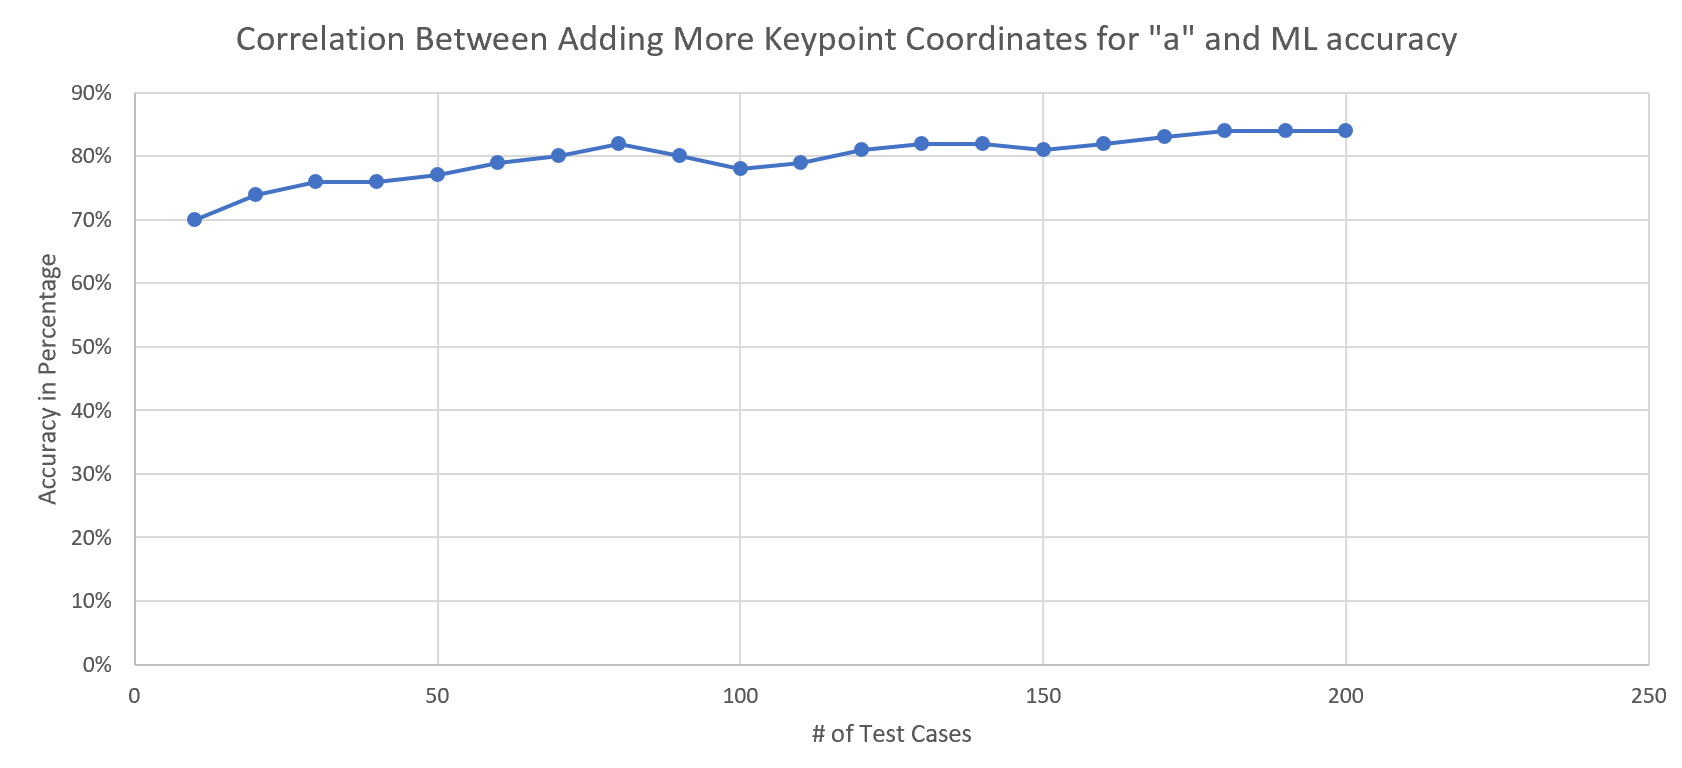
\includegraphics[width=\textwidth,height=0.4\textheight,keepaspectratio]{correlation.PNG} 
\caption{Correlation Graph} 
\label{Fig.Correlation} 
\end{figure}

The pictures above are some examples of our test for the robustness of the machine learning 
module following a rigorous evaluation process.. We introduced various types of noise and 
perturbations as our input for this test. This includes obscuring parts of the hand, changing
the lighting, and a different orientation. We measured the robustness using these conditions
and fine-tuned the model by retraining it using the perturbed data. Finally, we validated the
performance by testing with a different set of users, as seen above in the images, with different
hand sizes and gestures to help ensure that the model is robust and reliable for recognizing hand
gestures in a wide range of real-world scenarios.

\newpage
\section{Non-Functional Quality 2}

\begin{figure}[!ht]
\minipage{0.5\textwidth}
  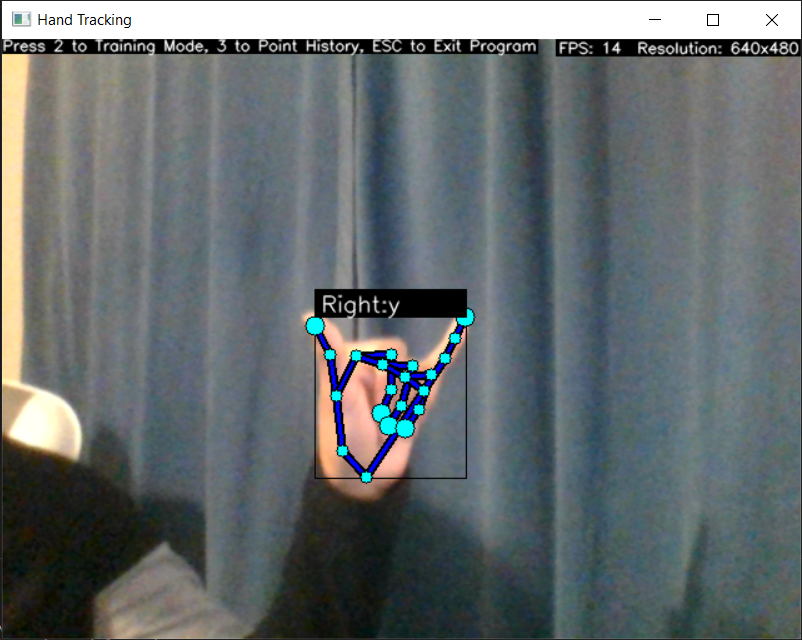
\includegraphics[width=\linewidth]{angled_y.png}
  \caption{Angled y}\label{fig:Angled y}
\endminipage\centering
\minipage{0.5\textwidth}
  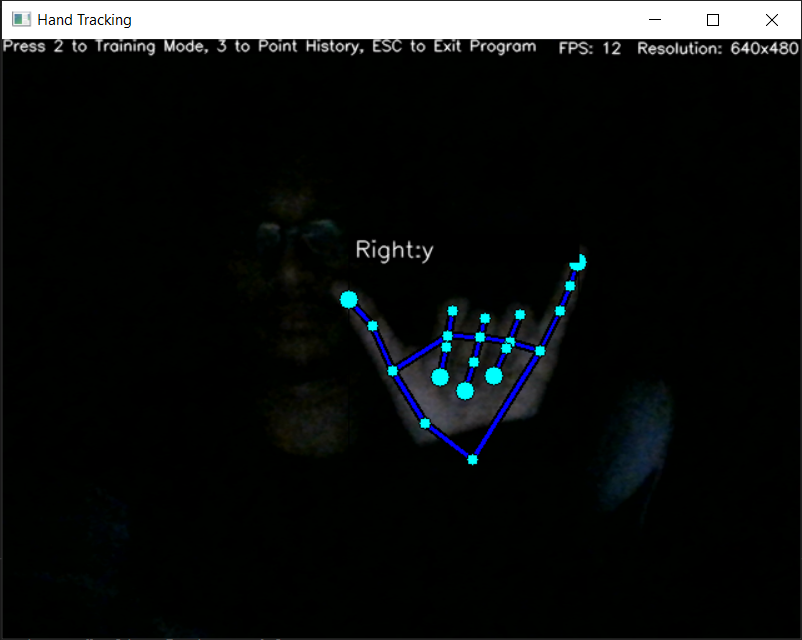
\includegraphics[width=\linewidth]{low_light_y.png}
  \caption{Low Light y}\label{fig:Low Light y}
\endminipage\hfill
\end{figure}

\begin{figure}[!ht]
\minipage{0.5\textwidth}
  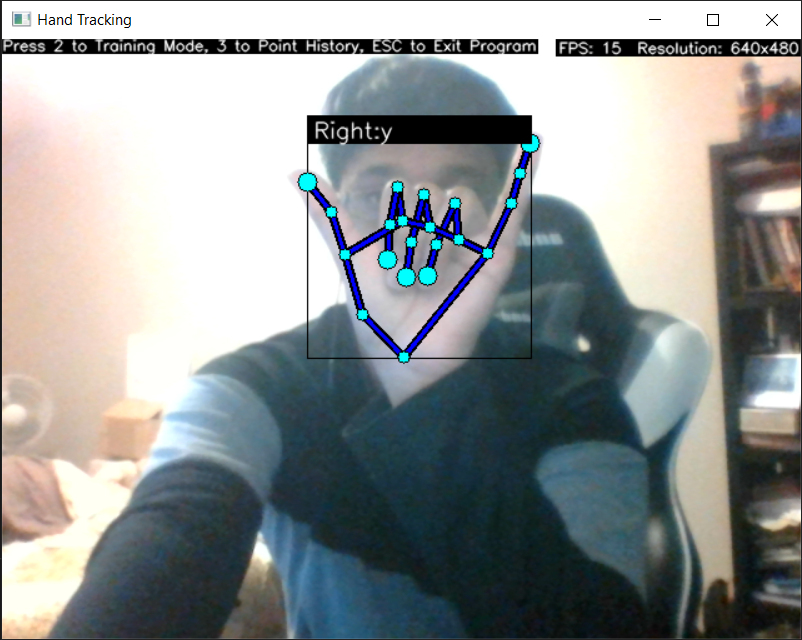
\includegraphics[width=\linewidth]{normal_y.png}
  \caption{Normal y}\label{fig:Normal y}
\endminipage\centering
\minipage{0.5\textwidth}
  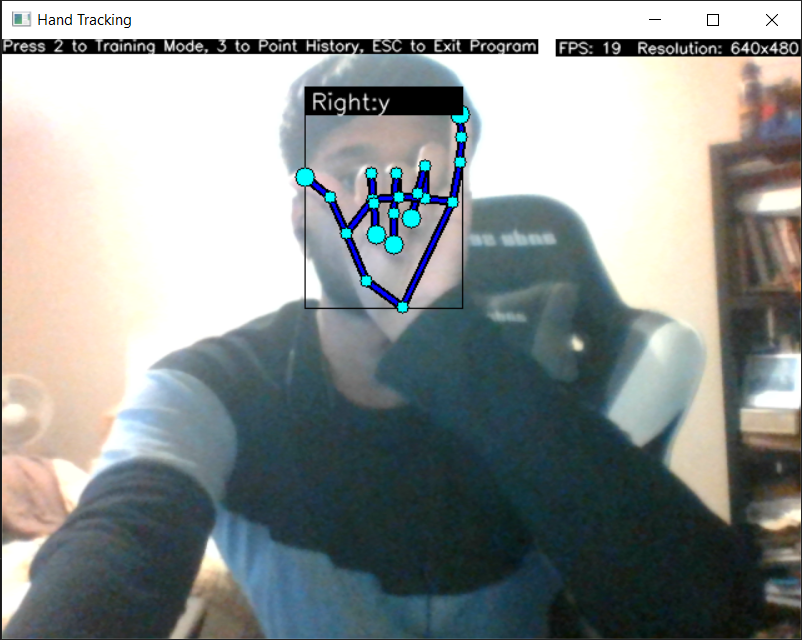
\includegraphics[width=\linewidth]{left_y.png}
  \caption{Tilted Left}\label{fig:Tilted Left}
\endminipage\hfill
\end{figure}

\begin{figure}[!ht]
\minipage{0.5\textwidth}
  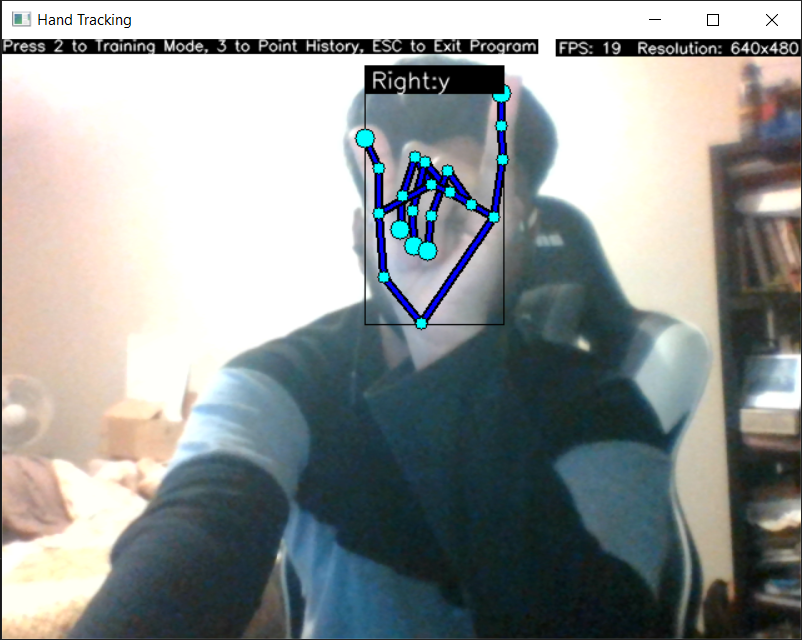
\includegraphics[width=\linewidth]{right_y.png}
  \caption{Tilted Right}\label{fig:Tilted Right}
\endminipage\hfill
\end{figure}
\minipage{1\textwidth}
~\\
The pictures above are some examples of our test for the robustness of the machine 
learning module following a rigorous evaluation process.. We introduced various types 
of noise and perturbations as our input for this test. This includes obscuring parts 
of the hand, changing the lighting, and a different orientation. We measured the robustness
using these conditions and fine-tuned the model by retraining it using the perturbed data. 
Finally, we validated the performance by testing with a different set of users, as seen above 
in the images, with different hand sizes and gestures to help ensure that the model is robust 
and reliable for recognizing hand gestures in a wide range of real-world scenarios.
\endminipage

\section{Changes due to Testing}

From the failures of test cases G2 and H2, it was determined that the program’s performance on a Raspberry Pi is inadequate; 
likely due to hardware limitations with single core processing. Thus, the approach that we decided to take was to rewrite the 
program such that the Raspberry Pi is able to utilize Python’s multiprocessing library to alleviate performance issues. As of 
writing this, this solution is still being worked on and is not guaranteed to work. There are also potentially other solutions 
to use slightly more powerful hardware such as mobile devices or another board, though the main concern would be the portability requirement NFR6.\\
~\\
In addition, from test cases D2 and D6, the program fails to detect the difference between its modes KeypointClassification 
(regular static gesture), PointHistoryClassification (motion gesture), and idle (where no gestures should be detected). At the 
moment, both modes operate at the same exact time which may cause confusion for the user and cause issues with the text to speech 
module. Therefore, changes to the program as a result of the tests would include a method that provides better distinction between 
the two modes.\\
~\\
Furthermore from the test cases for the training module, we encountered an oversight with how training would occur when signing with 
both hands. We have it currently set up so that you would press a key to record the coordinates of your hand gestures. But in doing so, 
we failed to realize how this would work when performing signs that required the use of both hands. As a result of this circumstance, we 
are now working on implementing a change to the GUI that enables automated recording of these gestures where a keypress will start a timer 
of 10 seconds then record a data point every 5 seconds. These values are subject to change and will be adjusted as needed.\\
~\\
From test case D1, we can conclude that the accuracy of the model for similar gestures is also one aspect that is inadequate in quality. 
Therefore the change that would be made based on non-functional quality 1, would be to add more data points such that the machine learning 
model is able to draw a distinction between similar gestures.

\section{Code Coverage Metrics}

\begin{figure}[h]
  \minipage{0.48\textwidth}
    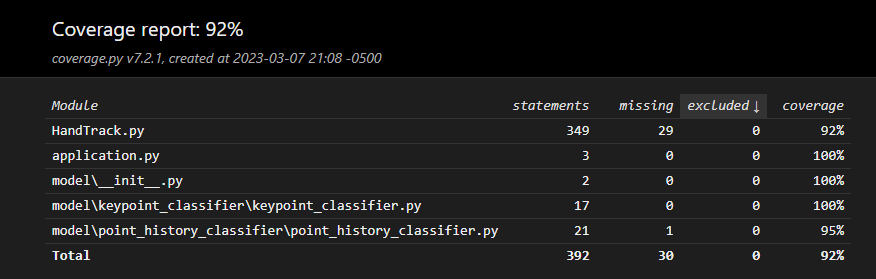
\includegraphics[width=\linewidth]{coverage_report_html.png}
    \caption{HTML Output}\label{fig:Coverage Report - HTML}
  \endminipage\hfill
  \minipage{0.48\textwidth}
    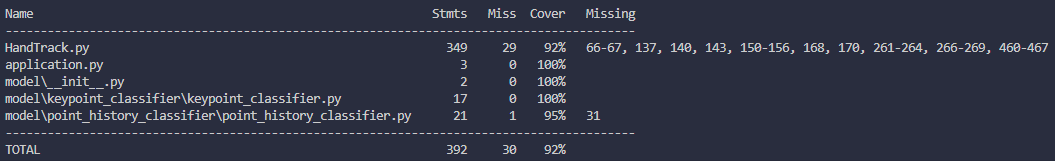
\includegraphics[width=\linewidth]{coverage_report_terminal.png}
    \caption{Terminal Output}\label{fig:Coverage Report - Terminal}
  \endminipage\hfill
\end{figure}\\
~\\
The images above are code coverage reports generated using Coverage.py which utilizes the PyTest Unit Testing Framework. \\
~\\
While the code coverage is not 100\%, it is reasonable enough at 92\% as not every single line of code will be hit upon execution. \\
~\\
This is especially true because there are portions of code which would require manual input from the user before they can be executed.


\bibliographystyle{plainnat}
\bibliography{../../refs/References}
~\\
The pictures above are some examples of our test for the robustness of the machine learning module following a 
rigorous evaluation process.. We introduced various types of noise and perturbations as our input for this test.
 This includes obscuring parts of the hand, changing the lighting, and a different orientation. We measured 
 the robustness using these conditions and fine-tuned the model by retraining it using the perturbed data. 
 Finally, we validated the performance by testing with a different set of users, as seen above in the images,
  with different hand sizes and gestures to help ensure that the model is robust and reliable for recognizing 
  hand gestures in a wide range of real-world scenarios.

\newpage{}
\section*{Appendix --- Reflection}

The information in this section will be used to evaluate the team members on the
graduate attribute of Reflection.  Please answer the following question:

\begin{enumerate}
  \item In what ways was the Verification and Validation (VnV) Plan different
  from the activities that were actually conducted for VnV?  If there were
  differences, what changes required the modification in the plan?  Why did
  these changes occur?  Would you be able to anticipate these changes in future
  projects?  If there weren't any differences, how was your team able to clearly
  predict a feasible amount of effort and the right tasks needed to build the
  evidence that demonstrates the required quality?  (It is expected that most
  teams will have had to deviate from their original VnV Plan.)\\

  Robert Zhu: One of the things we didn’t consider during the VnV plan was how the 
  GUI would be created and tested. During the VnV planning, the scope of the plan was 
  focused on machine learning and the newly purchased Raspberry Pi that required many 
  test cases to ensure that the gestures would be correctly translated using the new 
  hardware. The GUI requirements were less critical during the development process, 
  however during testing, we needed to think about how the user is about to access 
  the different functions of the code and the issues that occur from it. In future 
  projects this should be anticipated since the user experience is an important 
  requirement especially in this project where providing visual feedback to the user 
  in real-time is necessary for improving their performance and accuracy in hand signs.\\
  
  Mirza Nafi Hasan: Many things had changed from our VnV Plan. In our VnV plan, a lot 
  of the test cases covered only the basic functionality of our project. Since we have 
  gotten into the development, we have started to realize the details that we would need 
  to focus on. For example, in our VnV plan, we have a test case for detecting hand 
  gestures (TC-MLFR1). However, we failed to consider the edge cases, like what happens
  if two joints are on top of each other? Or if two hands are on top of each other? We 
  were able to get a better idea of these edge cases once we had started writing the 
  code. We would likely be able to identify some more tests we need to account for 
  before starting development for future projects.\\

  Kelvin Huynh: When we created our VnV Plan, we mentioned the use of the PyTest framework for 
  the purposes of automated testing. However, at the time we failed to consider how we would create 
  specific unit tests and their pass/fail conditions. Given the time constraint on the creation of the 
  VnV report, we were not able to implement the use of this tool in full capacity. Instead, we opted to 
  just do manual testing while considering as many test cases as possible. In future projects, this issue 
  could easily be circumvented if we actively thought of potential test cases and developed automated testing 
  scripts during the development process as needed.\\
  
  Jiahui Chen: By cross referencing to the VnV plan, one of the differences is that the test cases written in the VnV plan did not cover all the modules or functionalities that need to be tested. They were too general and did not correspond to the specific modules.Therefore, in the VnV Report, we redesigned the test cases based on modules to make sure all the important testing criteria are covered. This problem happened because at the beginning of the development, we missed out some functionalities of the modules and they were added during the development process. And we also changed some of the functions for the device when we realized the initial ideas or design could not be implemented well. For example, the text-to-speech module was added to replace the external speaker and the testing for the text-to-speech module needs to be conducted. We might still anticipate some changes to testing plans or testing cases in the future with the continuous development and improvement of the device. But this can be easily solved by adding more testing cases for the new functions or modules.\\

  Zifan Meng: One of the differences between the VnV plan and the actual VnV process is that the VnV plan did not  account for the differentiation between static hand gestures and motion gestures. However, during the development process, we realized that differentiating static gestures and motion gestures was crucial, due to the fact that American Sign Language involves a large amount of motions. Therefore, the key point history mode was developed and implemented for recognizing and translating motions. Corresponding test plans are also designed and executed to test whether the program can detect motions. Although it is difficult to anticipate every potential change that could arise, this experience indicates the importance of carefully considering the requirements of the project. We will continue to develop modularized programs so that the program is flexible and adaptable for possible modifications.\\
  
  Runze Zhu: A difference we encountered was the use of the Raspberry Pi not being able to run our program to the same level as a desktop or laptop computer and it struggles with the demanding application. This can be due to the amount of memory and the speed of the SD card being used. In the future we can learn to anticipate these issues by considering a single-board computer such as the Nvidia Jetson Nano, which was specially designed for computer vision, machine learning and robotics. While they are more expensive, they offer more powerful hardware and better performance for our use cases.

\end{enumerate}

\end{document}
